\subsubsection{ISOMAP}

Se aplico el algoritmo ISOMAP descrito en la sección \ref{sec:isomap_theory} con los datos de índice de marginación para los años 2015 y 2020. En la figura \ref{fig:isompa_2d} se observa los resultados del algoritmo para el caso bidimensional para 8, 10, 12 y 14 vecinos.

\begin{figure}[H]
    \centering
    \begin{subfigure}{8.4cm}
        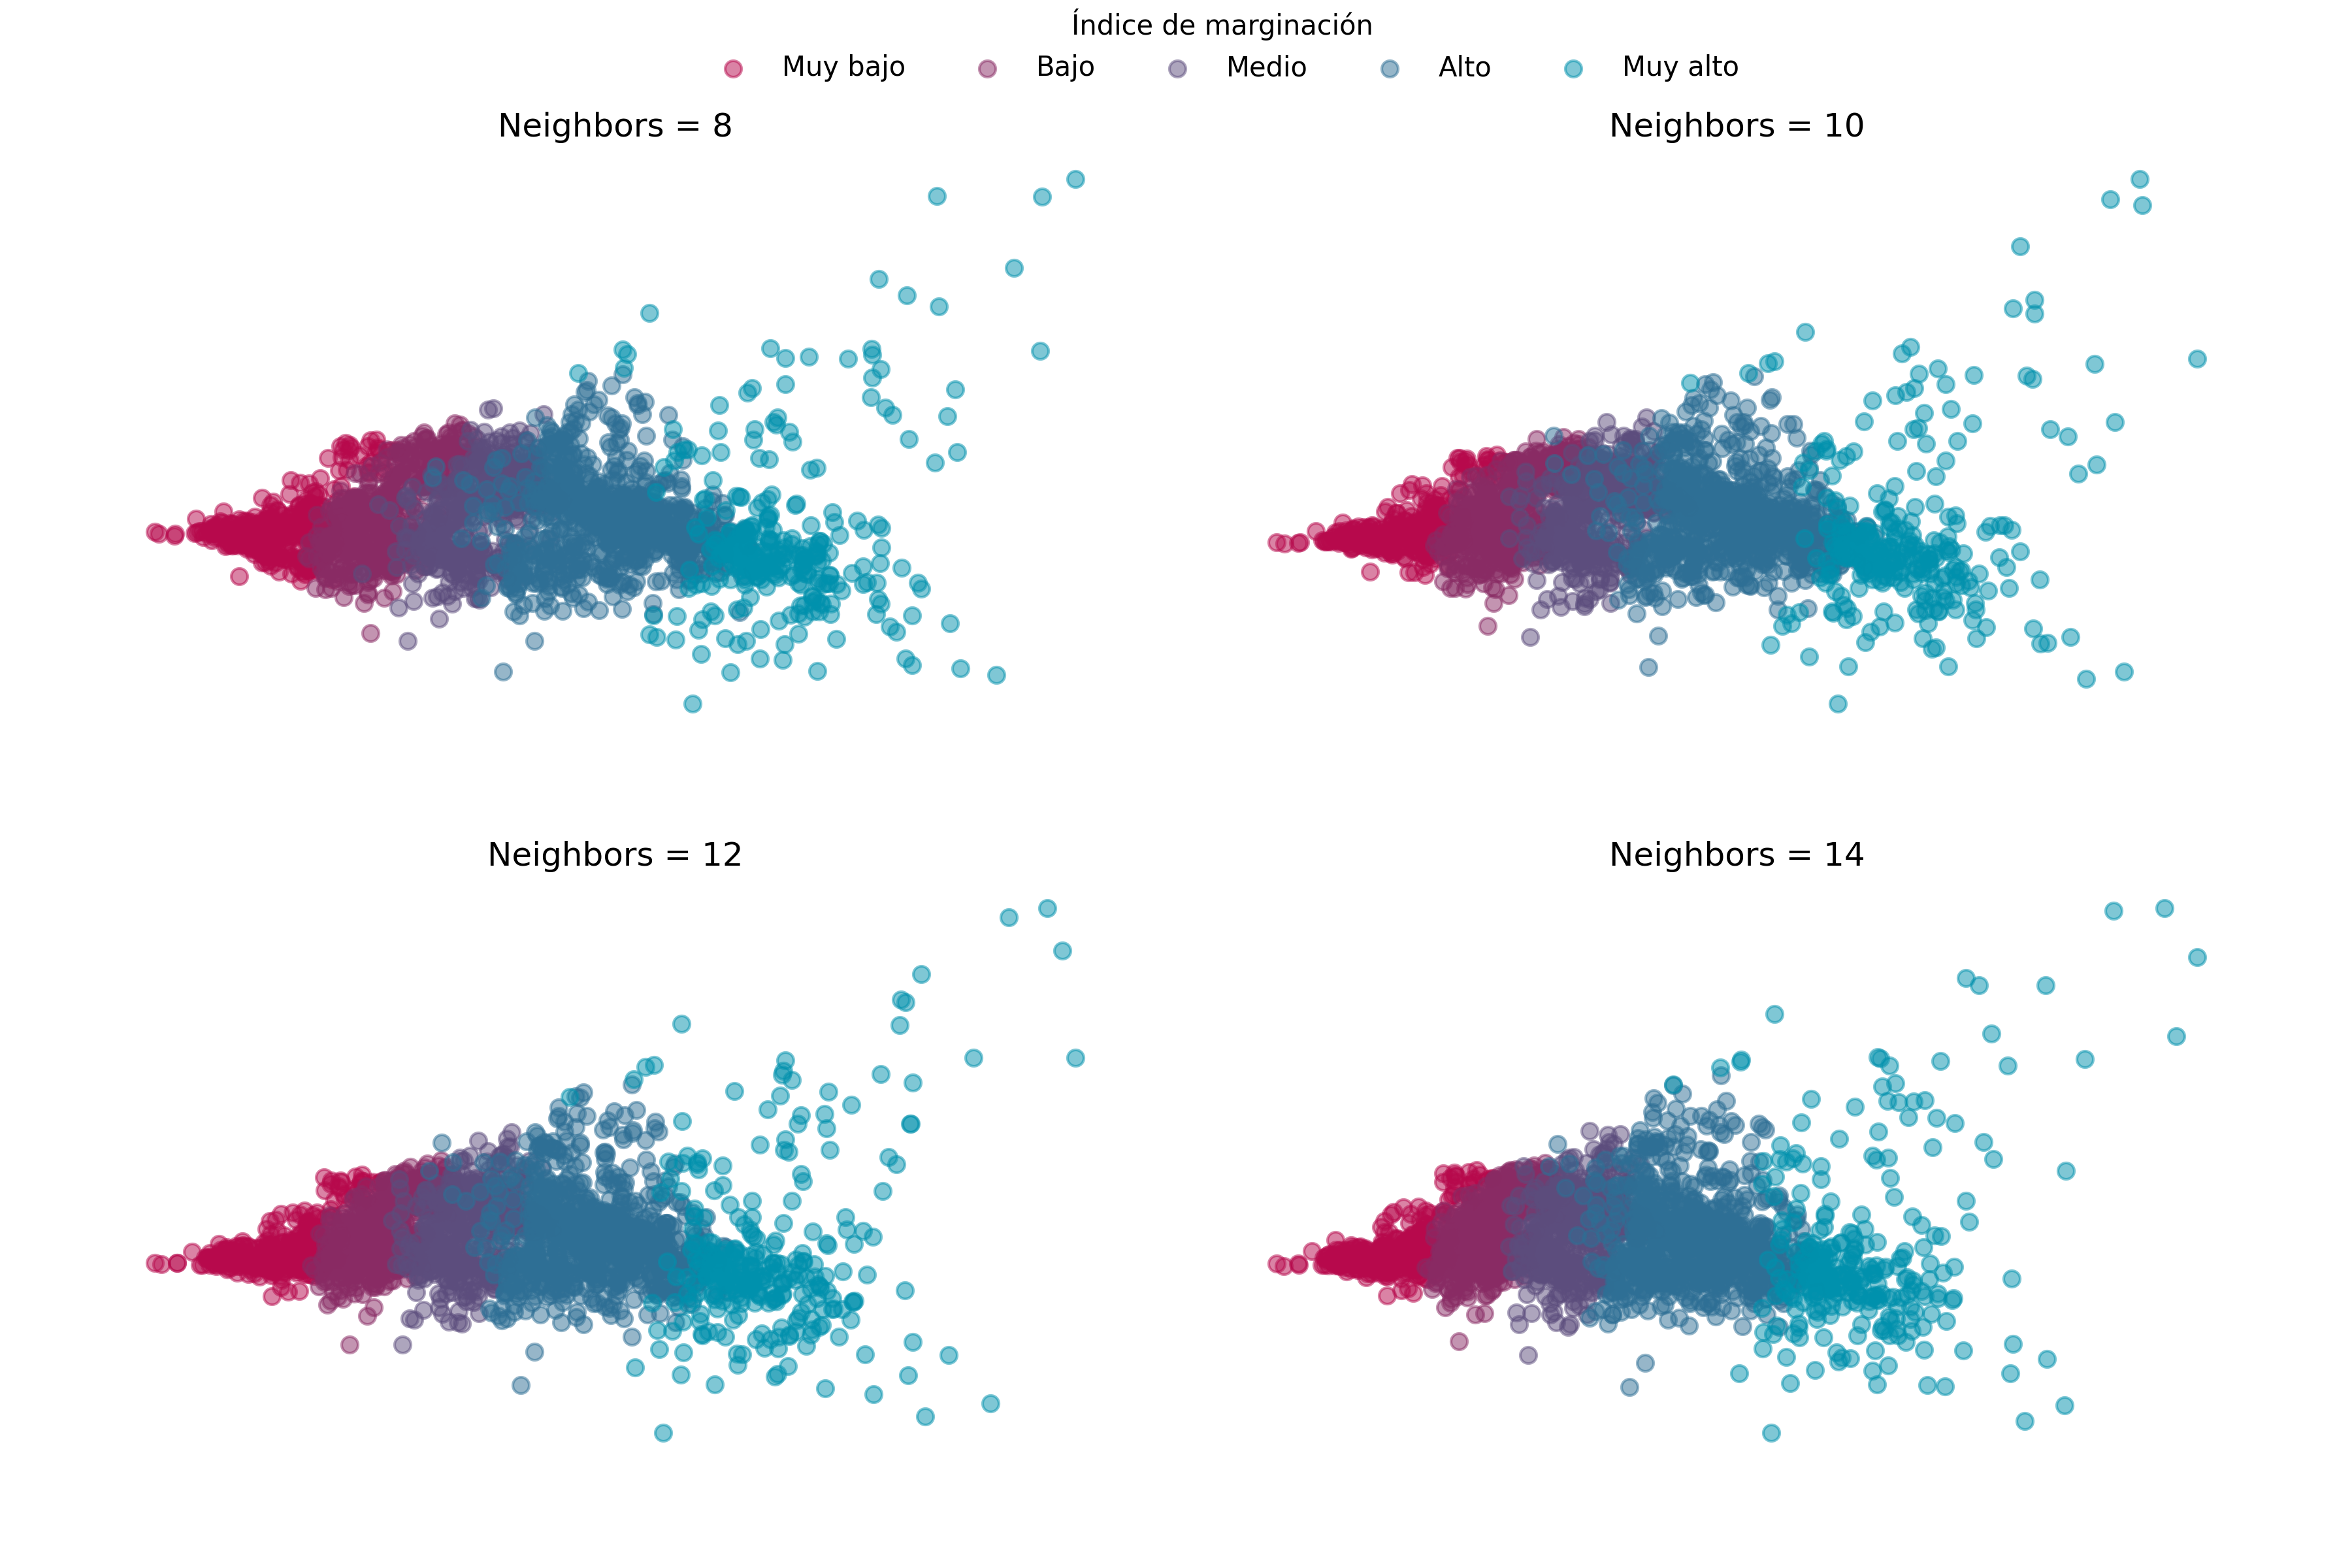
\includegraphics[width=1\linewidth]{Graphics/Data_2015/ISOMAP_2D.png}
        \caption{Datos 2015}
    \end{subfigure}
    \begin{subfigure}{8.4cm}
        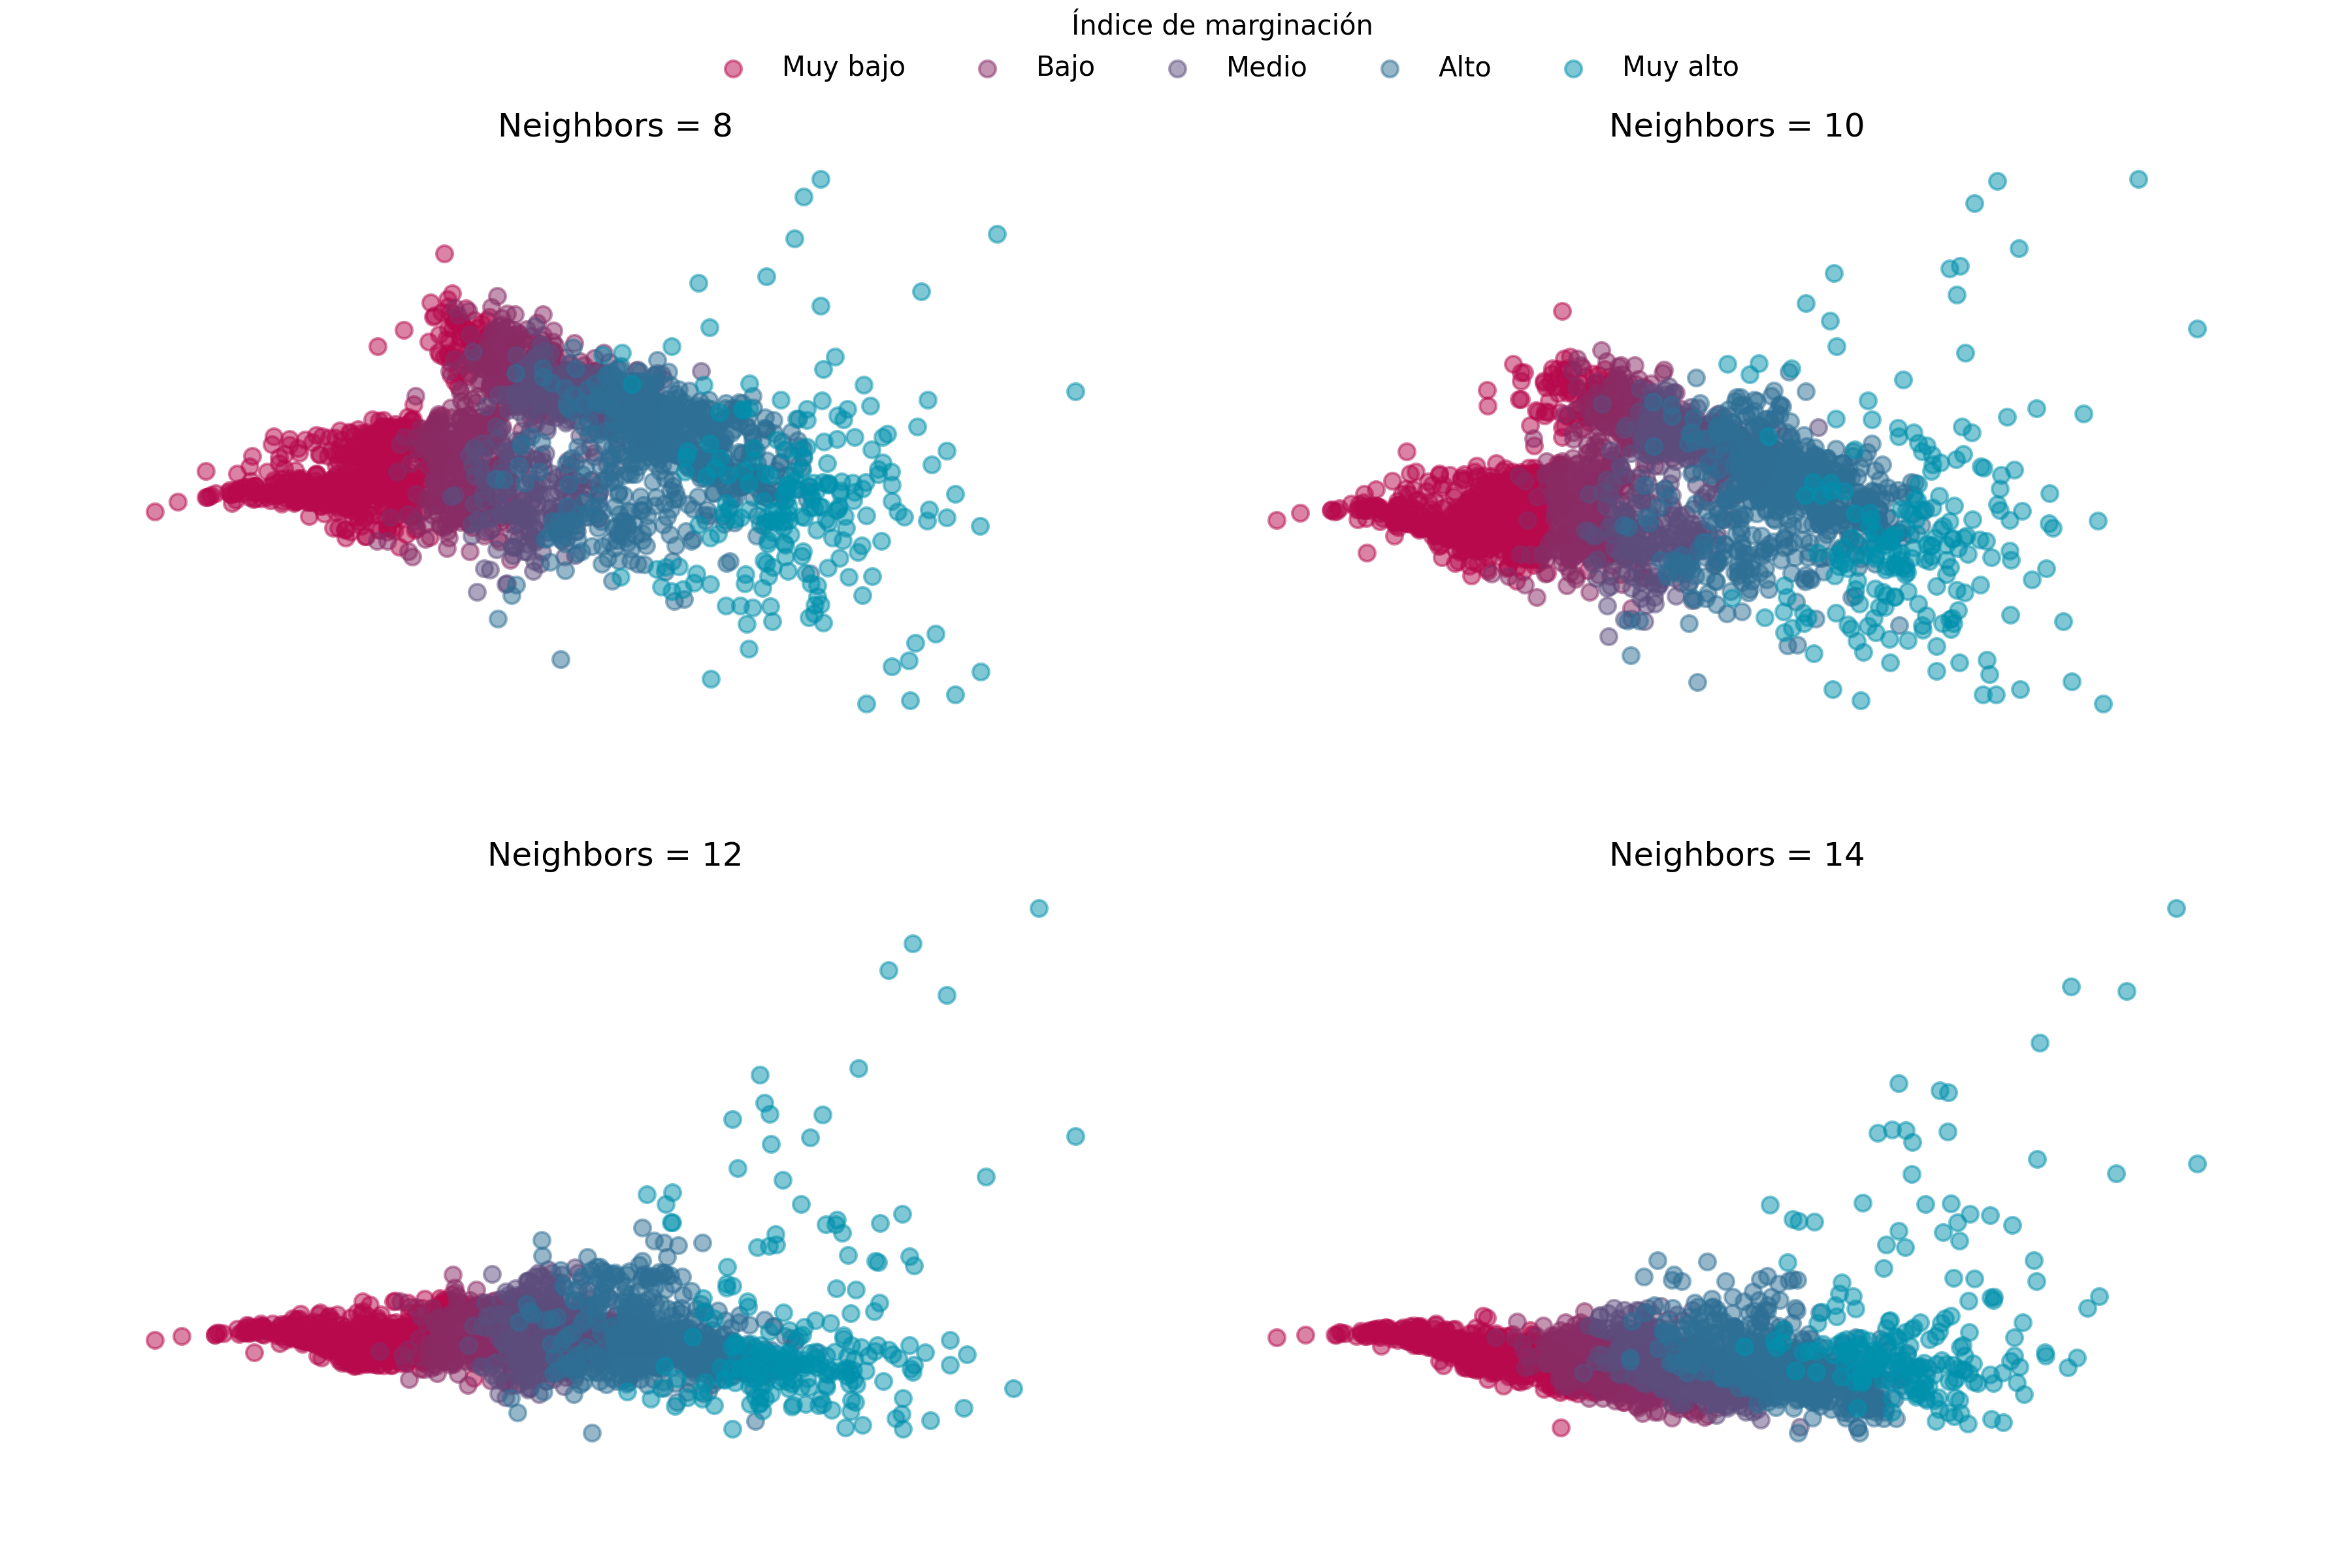
\includegraphics[width=1\linewidth]{Graphics/Data_2020/ISOMAP_2D.png}
        \caption{Datos 2020}
    \end{subfigure}
    \caption{Resultados de aplicar ISOMAP para el caso bidimensional para los datos de índice de marginación de los años 2015 y 2020.}
    \label{fig:isompa_2d}
\end{figure}

En la tabla \ref{table:isomap_results} se pueden descargar las visualizaciones tridimensionales de los resultados del algoritmo ISOMAP en el caso tridimensional para 8, 10, 12 y 14 vecinos para los años 2015 y 2020.

\begin{table}[H]
    \centering
    \begin{tabular}{lrr} \hline
        \multirow{2}{*}{Vecinos} & \multicolumn{2}{c}{Años}                                                                                                                                                                                                                                                \\ \cline{2-3}
                                 & 2015                                                                                                                               & 2020                                                                                                                               \\ \hline
        8                        & \href{https://github.com/giovannilopez9808/Reconocimiento_de_patrones_proyecto/raw/main/Graphics/Data_2015/ISOMAP_3D_8.mp4}{Link}  & \href{https://github.com/giovannilopez9808/Reconocimiento_de_patrones_proyecto/raw/main/Graphics/Data_2020/ISOMAP_3D_8.mp4}{Link}  \\
        10                       & \href{https://github.com/giovannilopez9808/Reconocimiento_de_patrones_proyecto/raw/main/Graphics/Data_2015/ISOMAP_3D_10.mp4}{Link} & \href{https://github.com/giovannilopez9808/Reconocimiento_de_patrones_proyecto/raw/main/Graphics/Data_2020/ISOMAP_3D_10.mp4}{Link} \\
        12                       & \href{https://github.com/giovannilopez9808/Reconocimiento_de_patrones_proyecto/raw/main/Graphics/Data_2015/ISOMAP_3D_12.mp4}{Link} & \href{https://github.com/giovannilopez9808/Reconocimiento_de_patrones_proyecto/raw/main/Graphics/Data_2020/ISOMAP_3D_12.mp4}{Link} \\
        14                       & \href{https://github.com/giovannilopez9808/Reconocimiento_de_patrones_proyecto/raw/main/Graphics/Data_2015/ISOMAP_3D_14.mp4}{Link} & \href{https://github.com/giovannilopez9808/Reconocimiento_de_patrones_proyecto/raw/main/Graphics/Data_2020/ISOMAP_3D_14.mp4}{Link} \\ \hline
    \end{tabular}
    \caption{Link de descarga para las visualizaciones tridimensionales de los resultados de ISOMAP para 8, 10, 12 y 14 vecinos en los años 2015 y 2020.}
    \label{table:isomap_results}
\end{table}